\documentclass[12pt]{article}

\usepackage{bm}
\usepackage{amsmath}
\usepackage{amsfonts}
\usepackage{amssymb}
\usepackage{graphicx}
\usepackage{colortbl}
\usepackage{xr}
\usepackage{hyperref}
\usepackage{longtable}
\usepackage{xfrac}
\usepackage{tabularx}
\usepackage{float}
\usepackage{siunitx}
\usepackage{booktabs}

%\usepackage{refcheck}
\usepackage{graphicx}

\hypersetup{
    bookmarks=true,         % show bookmarks bar?
      colorlinks=true,       % false: boxed links; true: colored links
    linkcolor=red,          % color of internal links (change box color with linkbordercolor)
    citecolor=green,        % color of links to bibliography
    filecolor=magenta,      % color of file links
    urlcolor=cyan           % color of external links
}

\usepackage{fullpage}

\begin{document}

\title{Test Report} 
\author{Alex Guerrero, Keyur Patel and Shafeeq Rabbani}
\date{\today}

\maketitle

\section{Revisions}
\begin{center}
	\begin{longtable}{ | r | p{4cm} | p{4cm} | p{4cm} |}
	\caption{Revisions} \\ \hline \label{TblInputVar} 
	Name & Date & Description\\ \hline
	Keyur Patel & 27/11/2015 &  Created Test Report latex file\\ \hline

	Keyur Patel & 27/11/2015 &  Added table template for unit testing AND info\\ \hline

	Alex Guerrero & 27/11/2015 & Edited Structural Testing\\ \hline
	
		Shafeeq Rabbani & 27/11/2015 & Edited Usability Testing\\ \hline
	\end{longtable}
\end{center}

\section{Structural (White Box) Testing}

\subsection{Unit Tests for Food}

\begin{center}
	\begin{longtable}{ | p{3cm} | p{4cm} | p{4cm} | p{2cm} |}
	\caption{Revisions} \\ \hline \label{TblInputVar} 
	Test Case & Initial State & Expected Output & Output\\ \hline
	testRandomPos.1 & foodA and foodB randomly placed & positions compared and not equal & pass  \\ \hline
	testRandomPos.2 & foodC randomly placed & || & pass  \\ \hline
	testRandomPos.3 & foodD randomly placed & || & pass  \\ \hline

	\end{longtable}
\end{center}

\tableofcontents
\newpage



\section{Features that were Tested}

\begin{itemize}
\item 1:The functional requirements of the product
\item 2:The classes and methods of the product (Model)
\item 3:The GUI of the product
\end{itemize}

\section{Testing Types}
Testing can be broken up into different types, which each have their own role in the testing the product. These test types should be utilized to comprehensively evaluate the quality of the product.
\subsection{Structural Testing}
Structural testing  is also known as white box testing. Structural tests are derived from the program's internal structure. It focuses on the nonfunctional requirements of the product. This type of testing shows errors that occur during the implementation by focusing on abnormal and extreme cases the product could encounter.
\subsection{Functional Testing}
Functional testing is also known as black box testing. Functional tests are derived from the functional requirements of the program. It focuses less on how the program works and more on the output of the system. These tests are focused on test cases where the product receives expected information.
\subsection{Static vs. Dynamic Testing}
Static testing simulate the dynamic environment and does not focus on code exectution. This testing involves code walkthroughs and requirements walkthroughs. Static testing is used prevalently in the design stage. In contrast, dynamic testing needs code to be executed. \newline\newline
Dynamic testing involves test cases to be run and checked against expected outcomes. A technique to save time during dynamic testing is to choose representative test cases. 
\subsection{Manual vs. Automatic Testing}
Manual testing is done by people. It involves code walkthroughs and inspection. \newline\newline
Automatic testing can usually be conducted by computers. The tools used to assist with automatic are unit testing tools for the respective programming language. Automatic testing relies on people for testing more qualitative aspects like GUI. 


\section{Automated Unit Testing}
For most of the applicable functions and methods, we tested for robustness by inputting abnormal conditions and extreme domains.
\subsection{Testing for Snake.py}
\begin{center}
	\begin{longtable}{ | r | p{4cm} | p{10cm} }
	\caption{Test Case for constructor} \\ \hline \label{TblInputVar} 
	\textbf{Function Tested} & Snake()\\ \hline
	\textbf{Preconditions} & none \\ \hline
	\textbf{Expected outcome} & a Snake() object is instantiated \\ \hline
	\textbf{Function Input} & none \\ \hline
	\textbf{Test Description} & This test asserts equality of two Snake() objects once in\\ \hline
	\textbf{Testing Type} & Correctness\\ \hline
	
	\end{longtable}
\end{center}

\begin{center}
	\begin{longtable}{ | r | p{4cm} | p{10cm} }
	\caption{Test Case for changeDir} \\ \hline \label{TblInputVar} 
	\textbf{Function Tested} & changeDir(newDirection)\\ \hline
	\textbf{Preconditions} & Snake object is already instantiated \\ \hline
	\textbf{Expected outcome} & The test object's direction is updated if it is a valid input \\ \hline
	\textbf{Function Input} & an integer from [-1,1,-2,2] \\ \hline
	\textbf{Test Description} & This test uses Snake objects in different directions and calls changeDir on them with all possible direciton inputs\\ \hline
	\textbf{Testing Type} & Correctness and Robustness\\ \hline
	
	\end{longtable}
\end{center}

\begin{center}
	\begin{longtable}{ | r | p{4cm} | p{10cm} }
	\caption{Test Case for grow} \\ \hline \label{TblInputVar} 
	\textbf{Function Tested} & grow\\ \hline
	\textbf{Preconditions} & there is an instantiated Snake() object \\ \hline
	\textbf{Expected outcome} & The snake's length increases by 1 \\ \hline
	\textbf{Function Input} & none \\ \hline
	\textbf{Test Description} & This test asserts equality between pregrown Snake objects and newly grown objects\\ \hline
	\textbf{Testing Type} & Correctness\\ \hline
	
	\end{longtable}
\end{center}

\begin{center}
	\begin{longtable}{ | r | p{4cm} | p{10cm} }
	\caption{Test Case for remove} \\ \hline \label{TblInputVar} 
	\textbf{Function Tested} & remove\\ \hline
	\textbf{Preconditions} & a Snake object is instantiated \\ \hline
	\textbf{Expected outcome} & every point in the snake after the inputted index is removed \\ \hline
	\textbf{Function Input} & integer value corresponding to the index \\ \hline
	\textbf{Test Description} & This test asserts equality between the length of a Snake object that has remove executed at various indexes and said indexes+1. This test also tests for abnormal and extreme values\\ \hline
	\textbf{Testing Type} & Correctness,Robustness\\ \hline
	
	\end{longtable}
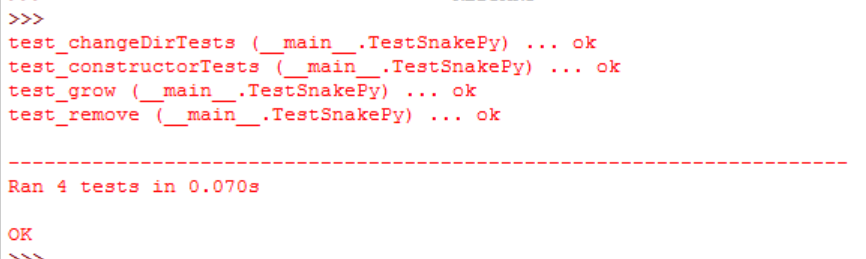
\includegraphics{testSnakeResults}\newline\newline
\end{center}

\subsection{Testing for MainMenu.py}
\begin{center}
	\begin{longtable}{ | r | p{4cm} | p{10cm} }
	\caption{Test Case for constructor} \\ \hline \label{TblInputVar} 
	\textbf{Function Tested} & MainMenu() \\ \hline
	\textbf{Preconditions} & none \\ \hline
	\textbf{Expected outcome} & a MainMenu object is instantiated \\ \hline
	\textbf{Function Input} & none \\ \hline
	\textbf{Test Description} & constructor equality test\\ \hline
	\textbf{Testing Type} & Correctness\\ \hline
	
	\end{longtable}
\end{center}

\begin{center}
	\begin{longtable}{ | r | p{4cm} | p{10cm} }
	\caption{Test Case for changeState} \\ \hline \label{TblInputVar} 
	\textbf{Function Tested} & changeState\\ \hline
	\textbf{Preconditions} & a MainMenu object has been instantiated \\ \hline
	\textbf{Expected outcome} & the state is updated if input is valid \\ \hline
	\textbf{Function Input} & string value corresponding to the new state \\ \hline
	\textbf{Test Description} & This test asserts equality between the inputted newState and the state of the MainMenu object after running changeState on it\\ \hline
	\textbf{Testing Type} & Correctness,Robustness\\ \hline
	
	\end{longtable}
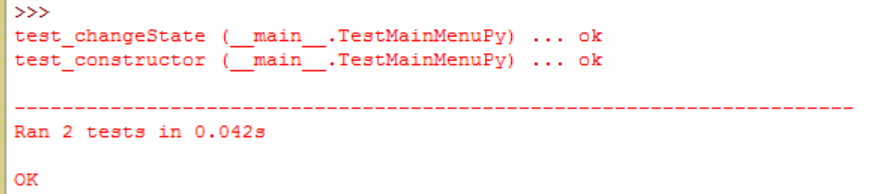
\includegraphics{testMainMenuResults}\newline\newline
\end{center}


\subsection{Testing for Food.py}
\begin{center}
	\begin{longtable}{ | r | p{4cm} | p{4cm} }
	\caption{Test Case for constructor} \\ \hline \label{TblInputVar} 
	Function Tested & Food()\\ \hline
	Preconditions & none \\ \hline
	Expected outcome & random x and y position \\ \hline
	Function Input & none \\ \hline
	Test Description & Assert that two food objects have different positions \\ \hline
	Testing Type & Correctness\\ \hline
	
	\end{longtable}
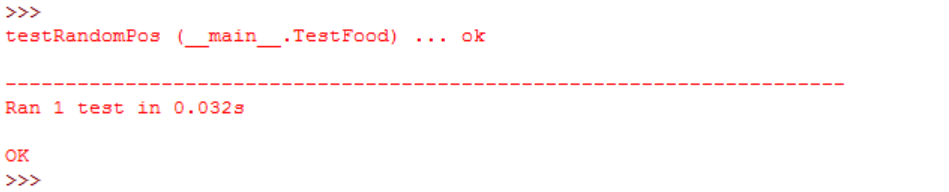
\includegraphics{testFoodResults}\newline\newline	
\end{center}

\subsection{Testing for PlayMap.py}
\begin{center}
	\begin{longtable}{ | r | p{4cm} | p{4cm} }
	\caption{Test Case for setDiff} \\ \hline \label{TblInputVar} 
	Function Tested & setDiff(difficulty)\\ \hline
	Preconditions & none \\ \hline
	Expected outcome & difficulty changes to number passed  \\ \hline
	Function Input & 0, 1, and 2 \\ \hline
	Test Description & Assert that difficult changes after being set\\ \hline
	Testing Type & Correctness\\ \hline
	
	\end{longtable}
\end{center}

\begin{center}
	\begin{longtable}{ | r | p{4cm} | p{4cm} }
	\caption{Test Case for didSnakeHitBoarder} \\ \hline \label{TblInputVar} 
	Function Tested & didSnakeHitBoarder()\\ \hline
	Preconditions & moving snake head to desired test location \\ \hline
	Expected outcome & Return true when snake hits border, False else  \\ \hline
	Function Input & none \\ \hline
	Test Description & Assert that function returns true only when snake hits border \\ \hline
	Testing Type & Correctness\\ \hline
	
	\end{longtable}
\end{center}

\begin{center}
	\begin{longtable}{ | r | p{4cm} | p{4cm} }
	\caption{Test Case for didSnakeHitSelf} \\ \hline \label{TblInputVar} 
	Function Tested & didSnakeHitSelf()\\ \hline
	Preconditions & moving snake head to desired test location \\ \hline
	Expected outcome & Return True when snake hits self, False else \\ \hline
	Function Input & none \\ \hline
	Test Description & Assert that function returns true only when snake hits self \\ \hline
	Testing Type & Correctness\\ \hline
	
	\end{longtable}
\end{center}
	
\begin{center}
	\begin{longtable}{ | r | p{4cm} | p{4cm} }
	\caption{Test Case for isSnakeDead} \\ \hline \label{TblInputVar} 
	Function Tested & isSnakeDead()\\ \hline
	Preconditions & moving snake head to desired test location \\ \hline
	Expected outcome & Return True when snake dies, False else \\ \hline
	Function Input & none \\ \hline
	Test Description & Assert that snake dies when it hits itself or a border\\ \hline
	Testing Type & Correctness\\ \hline
	
	\end{longtable}
\end{center}

\begin{center}
	\begin{longtable}{ | r | p{4cm} | p{4cm} }
	\caption{Test Case for updateState} \\ \hline \label{TblInputVar} 
	Function Tested & updateState()\\ \hline
	Preconditions & snake and food position \\ \hline
	Expected outcome & Snake grows by 1 when it eats food, remains the same length else \\ \hline
	Function Input & none \\ \hline
	Test Description & Assert that playMap updates correctly \\ \hline
	Testing Type & Correctness\\ \hline
	
	\end{longtable}
\end{center}

\begin{center}
	\begin{longtable}{ | r | p{4cm} | p{4cm} }
	\caption{Test Case for getCurrentState} \\ \hline \label{TblInputVar} 
	Function Tested & getCurrentState()\\ \hline
	Preconditions & moving snake head to desired test location \\ \hline
	Expected outcome & Return -1 when dead, an array of state variables else \\ \hline
	Function Input & none \\ \hline
	Test Description & Assert that getCurrentState returns correct value\\ \hline
	Testing Type & Correctness\\ \hline
	
	\end{longtable}
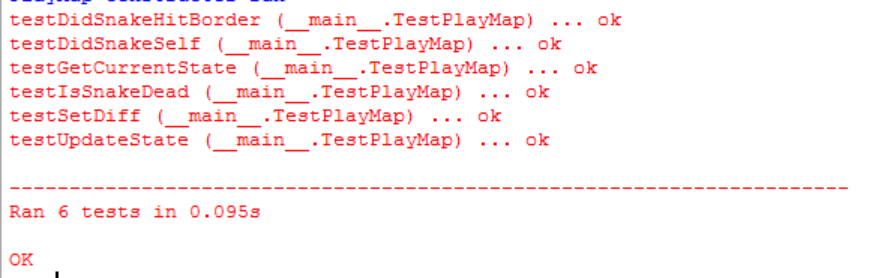
\includegraphics{testPlayMapResults}\newline\newline
\end{center}


\subsection{Testing for GamePause.py}
\begin{center}
	\begin{longtable}{ | r | p{4cm} | p{4cm} }
	\caption{Test Case for updateState} \\ \hline \label{TblInputVar} 
	Function Tested & updateState(score)\\ \hline
	Preconditions & none \\ \hline
	Expected outcome & Score variable in pause updates to number passed  \\ \hline
	Function Input & 21 \\ \hline
	Test Description & Assert that score changes after being updated\\ \hline
	Testing Type & Correctness\\ \hline
	
	\end{longtable}
\end{center}

\begin{center}
	\begin{longtable}{ | r | p{4cm} | p{4cm} }
	\caption{Test Case for getCurrentState} \\ \hline \label{TblInputVar} 
	Function Tested & getCurrentState()\\ \hline
	Preconditions & none \\ \hline
	Expected outcome & Return an array consisting of score, and the 4 buttons on the display  \\ \hline
	Function Input & none \\ \hline
	Test Description & Assert that function returns the proper array of items \\ \hline
	Testing Type & Correctness\\ \hline
	
	\end{longtable}
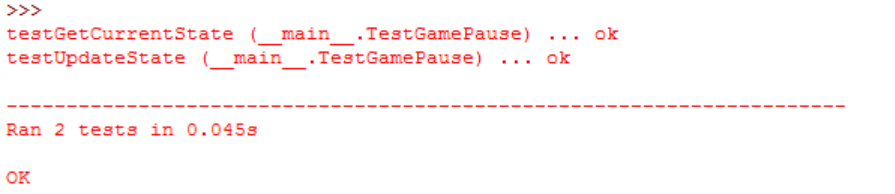
\includegraphics{testGamePauseResults}\newline\newline
\end{center}

\subsection{Testing for GameOver.py}
\begin{center}
	\begin{longtable}{ | r | p{4cm} | p{4cm} }
	\caption{Test Case for updateState} \\ \hline \label{TblInputVar} 
	Function Tested & updateState(score)\\ \hline
	Preconditions & none \\ \hline
	Expected outcome & Score variable in pause updates to number passed  \\ \hline
	Function Input & 21 \\ \hline
	Test Description & Assert that score changes after being updated\\ \hline
	Testing Type & Correctness\\ \hline
	
	\end{longtable}

\end{center}

\begin{center}
	\begin{longtable}{ | r | p{4cm} | p{4cm} }
	\caption{Test Case for getCurrentState} \\ \hline \label{TblInputVar} 
	Function Tested & getCurrentState()\\ \hline
	Preconditions & none \\ \hline
	Expected outcome & Return an array consisting of score, and the 2 buttons on the display  \\ \hline
	Function Input & none \\ \hline
	Test Description & Assert that function returns the proper array of items \\ \hline
	Testing Type & Correctness\\ \hline
	
	\end{longtable}
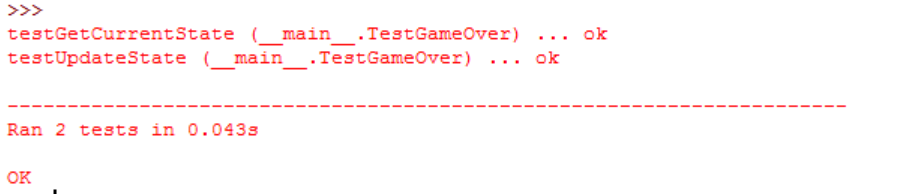
\includegraphics{testGameOverResults}\newline\newline
\end{center}


\section{Testing functional requirements}
\section{Usability Testing}
Usability testing is carried get response from gamers on their experience of the game. Testing
was carried by allowing youth between the age of 18 to 25. The comments and ratings given
by this focus group reflect the interests and needs of youth of today.

\begin{center}
	\begin{longtable}{ | l | p{8cm} | p{8cm}|}
	\caption{User 1} \\ \hline \label{TblUsr1} 
	Number of times played & 5 \\\hline
	Rate entertainment (from 1 to 10) &8 \\\hline
	Rate Power Up feature (from 1 to 10) &11 \\\hline
	Rate graphics (from 1 to 10) & 8 \\ \hline
	Suggested Improvements & There must be a way of knowing which difficulty level has been chosen. Response of keys
was slow. The game would be more interest-
ing had it been multiplayer.\\ \hline
	\end{longtable}

	\begin{longtable}{ | l | p{8cm} | p{8cm}|}
	\caption{User 2} \\ \hline \label{TblUsr2} 
	Number of times played & 2  \\ \hline
	Rate entertainment (from 1 to 10) & 7.5 \\ \hline
	Rate Power Up feature (from 1 to 10) & 10 \\ \hline
	Rate graphics (from 1 to 10) & 8 \\ \hline
	Suggested Improvements & There should be more menu options.\\ \hline
	\end{longtable}

	\begin{longtable}{ | l | p{8cm} | p{8cm}|}
	\caption{User 3} \\ \hline \label{TblUsr3} 
	Number of times played & 6  \\ \hline
	Rate entertainment (from 1 to 10) & 6 \\ \hline
	Rate Power Up feature (from 1 to 10) & 7 \\ \hline
	Rate graphics (from 1 to 10) & 7 \\ \hline
	Suggested Improvements & \ The game should be more colorful. \\hline
	\end{longtable}

	\begin{longtable}{ | l | p{8cm} | p{8cm}|}
	\caption{User 4} \\ \hline \label{TblUsr4} 
	Number of times played & 5 \\ \hline
	Rate entertainment (from 1 to 10) & 6 \\ \hline
	Rate Power Up feature (from 1 to 10) & 7 \\ \hline
	Rate graphics (from 1 to 10) & 2  \\ \hline
	Suggested Improvements & There appears to be a lag. Make the score board at the top of the screen more noticeable.\\ \hline
	\end{longtable}

	\begin{longtable}{ | l | p{8cm} | p{8cm}|}
	\caption{User 5} \\ \hline \label{TblUsr5} 
	Number of times played & 2 \\ \hline
	Rate entertainment (from 1 to 10) & 7.5 \\ \hline
	Rate Power Up feature (from 1 to 10) & 10 \\ \hline
	Rate graphics (from 1 to 10) & 8 \\ \hline
	Suggested Improvements & There should be more options in the options menu. \\ \hline
	\end{longtable}

	\begin{longtable}{ | l | p{8cm} | p{8cm}|}
	\caption{User 6}  \\ \hline \label{TblUsr6} 
	Number of times played &  8 \\ \hline
	Rate entertainment (from 1 to 10) & 7 \\ \hline
	Rate Power Up feature (from 1 to 10) & 8 \\ \hline
	Rate graphics (from 1 to 10) & 5  .\\ \hline
	Suggested Improvements & The top ten scores ever should be saved \\ \hline
	\end{longtable}

	\begin{longtable}{ | l | p{8cm} | p{8cm}|}
	\caption{User 7} \\ \hline \label{TblUsr7} 
	Number of times played & 3 \\ \hline
	Rate entertainment (from 1 to 10) & 6 \\ \hline
	Rate Power Up feature (from 1 to 10) & 2 \\ \hline
	Rate graphics (from 1 to 10) & 1 \\ \hline
	Suggested Improvements & Fix the lag. Add more modes such as a 			mode to make the snake go through one wall and come out from the 		other side. Add obstacles for the snake. Reward 'bonus' food 			points which appear for 5 seconds and disappear if not eaten by 		snake within this time. \\ \hline
	\end{longtable}
\end{center}
\newpage
\section{GUI Testing}

All features of the graphical user interface were tested to see that they correctly respond to the inputs let they be from mouse or the keyboard. 
\\
\textbf{Test Input:} The program is first run.\\
\textbf{Expected:} The option menu appears.\\
\textbf{Output:} Pass.\\
\pagebreak
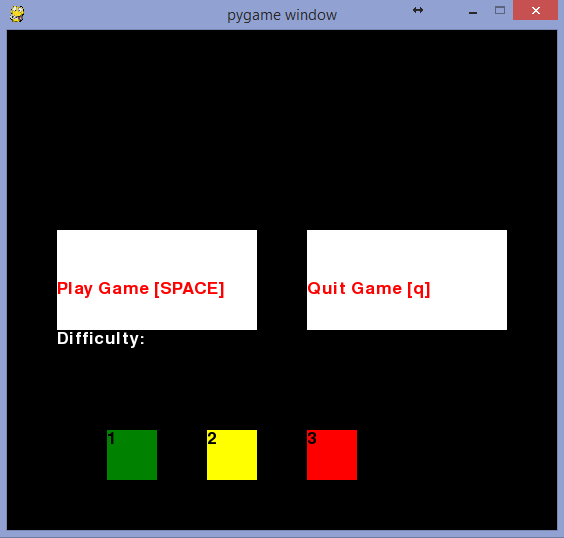
\includegraphics[width=\textwidth]{startmenu.png}\\
\textbf{Test Input:} In the option menu, Play Game is clicked or the space bar is pressed.\\
\textbf{Expected:} The snake game begins.\\
\textbf{Output:} Pass.\\
\pagebreak
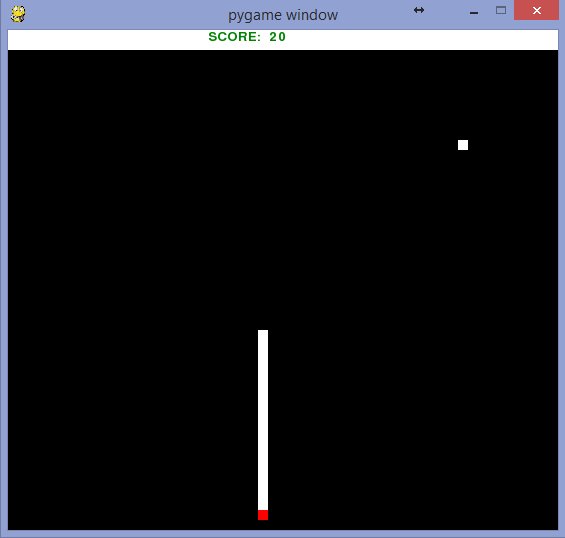
\includegraphics[width=\textwidth]{startgame.png}\\
\\
\textbf{Test Input:} In the game, UP arrow key is pressed while the snake is horizontally positioned.\\
\textbf{Expected:} The snake turns up.\\
\textbf{Output:} Pass.\\
\pagebreak
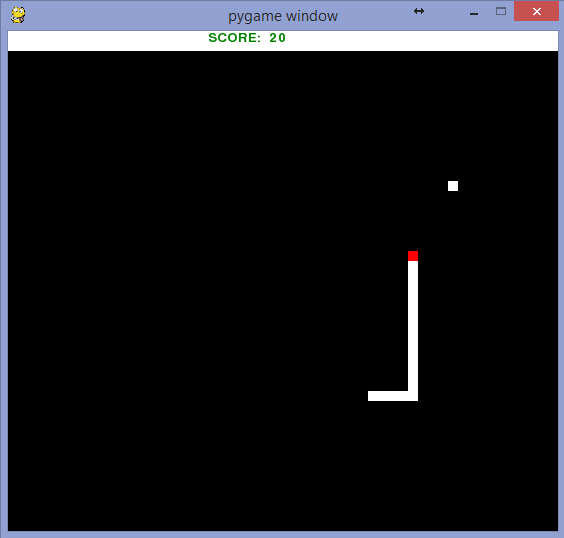
\includegraphics[width=\textwidth]{snakeup.png}
\\
\textbf{Test Input:} The DOWN arrow key is pressed when the snake is horizontally positioned.\\
\textbf{Expected:} The snake turns down.\\
\textbf{Output:} Pass.\\
\pagebreak
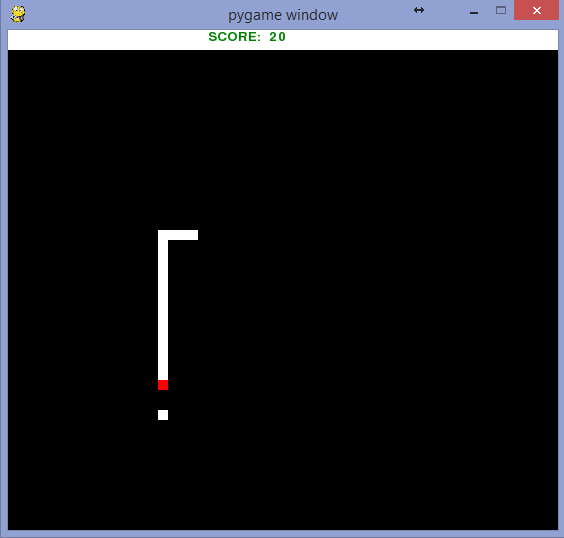
\includegraphics[width=\textwidth]{snakedown.png}\\
\\
\textbf{Test Input:} the RIGHT arrow key is pressed when the snake vertically positioned.\\
\textbf{Expected:} The snake turns right.\\
\textbf{Output:} Pass.\\
\pagebreak
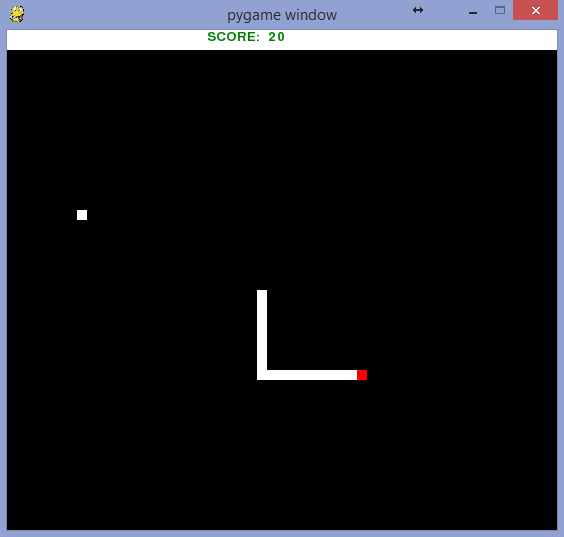
\includegraphics[width=\textwidth]{snakeright.png}\\
\\
\textbf{Test Input:} The LEFT arrow key is pressed when the snake is vertically positioned.\\
\textbf{Expected:} The snake turns left.\\
\textbf{Output:} Pass.\\
\pagebreak
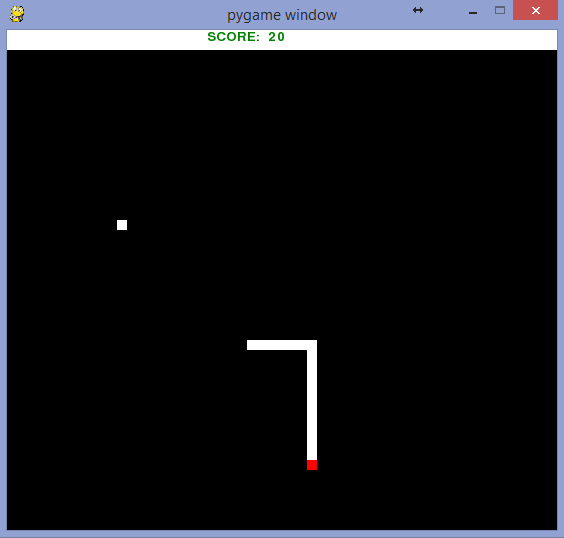
\includegraphics[width=\textwidth]{snakeleft.png}\\
\\
\textbf{Test Input:} The snake crashes into itself.\\
\textbf{Expected:} ,It's Power up will be used, the size of the snake will shrink and the red head disappears.\\
\textbf{Output:} Pass.\\
\pagebreak
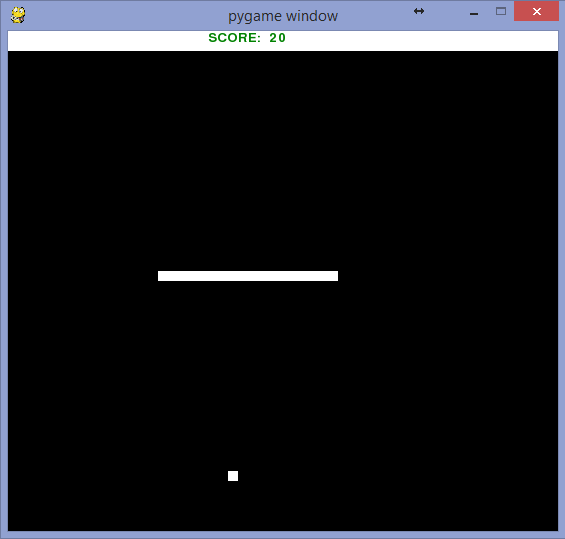
\includegraphics[width=\textwidth]{powerup.png}\\
\\
\textbf{Test Input:} The snake crashes the border.\\
\textbf{Expected:} The Game Over screen pops up and the game ends. The screen displays the score and options to either restart or quit the game.\\
\textbf{Output:} Pass.\\
Before: \pagebreak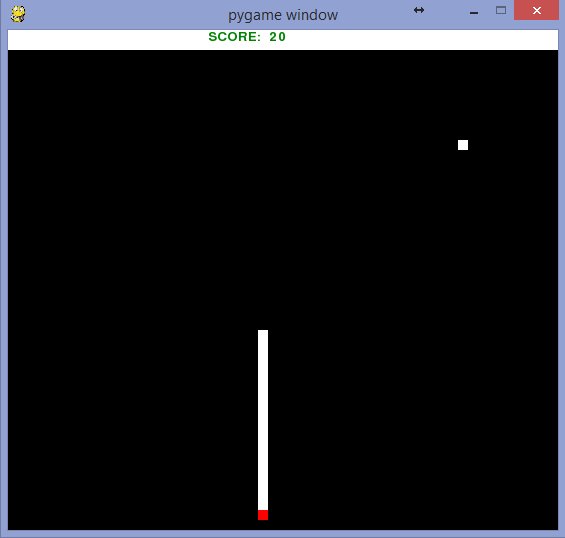
\includegraphics[width=\textwidth]{startgame.png}\\

After: \pagebreak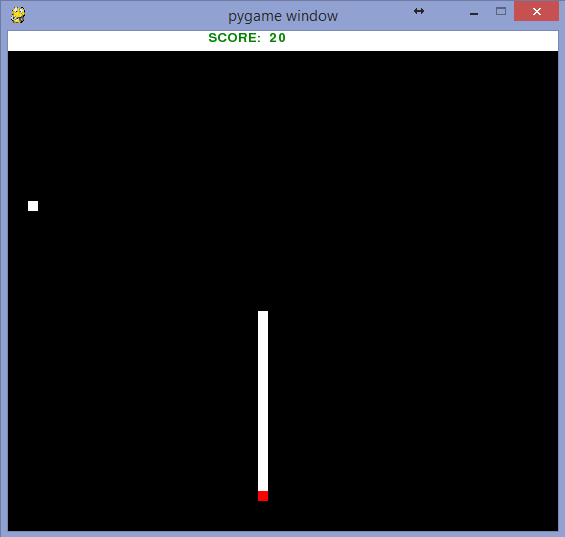
\includegraphics[width=\textwidth]{crash.png}\\
\\
\textbf{Test Input:} In the game over menu, the space bar is pressed.\\
\textbf{Expected:} The game successfully restarts.\\
\textbf{Output:}  Pass.\\
\pagebreak
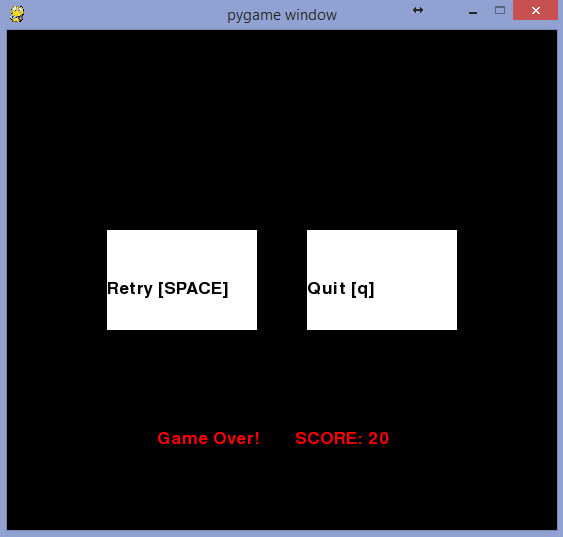
\includegraphics[width=\textwidth]{restart.png}
\\
\textbf{Test Input:} The letter 'q is pressed in the options menu, during the game and in the game over menu. \\
\textbf{Expected:} Pressing q quits the program.\\
\textbf{Output:} Pass.\\
Program window successfully closed in all three test cases.\\

\end{document}
